% =====================================================================
%  B.Tech. Project Report (CSP-400A), Department of CSE, IIT Roorkee
%  Memory-Efficient Rectangular Universalization in the OBSCURE Obfuscator
%
%  Build:  pdflatex BTP_Report.tex   (run twice for the table of contents)
%  Every value shown in [red brackets] is a placeholder to be filled in.
%  Every measured number comes from ../verification/results/*/summary.json
% =====================================================================
\documentclass[12pt,a4paper,oneside]{report}

% ---------------------------------------------------------------- packages
\usepackage[T1]{fontenc}
\usepackage[utf8]{inputenc}
\usepackage{mathptmx}                 % Times New Roman, as in the template
\usepackage[a4paper,left=1in,right=1in,top=1in,bottom=1in,headheight=15pt]{geometry}
\usepackage{setspace}
\usepackage{fancyhdr}
\usepackage{titlesec}
\usepackage{graphicx}
\usepackage{booktabs}
\usepackage{tabularx}
\usepackage{array}
\usepackage{multirow}
\usepackage{longtable}
\usepackage[font=small,labelfont=bf,skip=6pt]{caption}
\usepackage{float}
\usepackage{xcolor}
\usepackage{listings}
\usepackage{enumitem}
\usepackage{amsmath}
\usepackage{tikz}
\usetikzlibrary{arrows.meta,positioning,shapes.geometric,fit,calc,backgrounds}
\usepackage{tocloft}
\usepackage[hidelinks]{hyperref}

% ---------------------------------------------------------------- layout (template: TNR 12 pt, 1.5 spacing, justified)
\setstretch{1.2}
\setlength{\parskip}{4pt}
\setlength{\intextsep}{8pt}
\setlength{\textfloatsep}{8pt}
\captionsetup{skip=4pt}
\setlength{\parindent}{0pt}
\setlength{\emergencystretch}{2em}
\setlist{itemsep=2pt,topsep=4pt}

\definecolor{ink}{HTML}{1F1F1E}
\definecolor{muted}{HTML}{5F5E5A}
\definecolor{accent}{HTML}{2A78D6}
\definecolor{accent2}{HTML}{EB6834}
\definecolor{accent3}{HTML}{1BAF7A}
\definecolor{codebg}{HTML}{F5F4F0}
\definecolor{todo}{HTML}{C62828}

% placeholders for information we do not have (never invented)
\newcommand{\ph}[1]{\textcolor{todo}{[#1]}}
% terminal screenshot: #1 image file (the original terminal screenshot, trimmed only in
% height, so the prompt and the command that was run are visible), #2 the command (for
% reference only), #3 caption
\newcommand{\screenshot}[3]{%
  \begin{figure}[H]\centering
  \IfFileExists{figures/#1}{\includegraphics[width=\textwidth]{figures/#1}}{%
  \fbox{\begin{minipage}[c][4.2cm][c]{0.9\textwidth}\centering\small
  \textcolor{todo}{\textbf{[Screenshot to be inserted: figures/\detokenize{#1}]}}\end{minipage}}}
  \caption{#3}\end{figure}}

% chapter headings like the template: "Chapter-1: Introduction"
\titleformat{\chapter}[display]{\normalfont\bfseries\centering}
  {\Large Chapter-\thechapter}{6pt}{\LARGE}
\titlespacing*{\chapter}{0pt}{-40pt}{14pt}
\titleformat{\section}{\normalfont\large\bfseries}{\thesection}{0.8em}{}
\titlespacing*{\section}{0pt}{10pt}{3pt}
\titleformat{\subsection}{\normalfont\normalsize\bfseries}{\thesubsection}{0.8em}{}
\titlespacing*{\subsection}{0pt}{7pt}{2pt}
\titleformat{\subsubsection}{\normalfont\normalsize\bfseries\itshape}{\thesubsubsection}{0.8em}{}

% headers and footers
\pagestyle{fancy}
\fancyhf{}
\fancyhead[L]{\small\itshape\nouppercase{\leftmark}}
\fancyhead[R]{\small\itshape B.Tech. Project Report}
\fancyfoot[C]{\thepage}
\renewcommand{\headrulewidth}{0.4pt}
\fancypagestyle{plain}{\fancyhf{}\fancyfoot[C]{\thepage}\renewcommand{\headrulewidth}{0pt}}
\renewcommand{\chaptermark}[1]{\markboth{Chapter \thechapter: #1}{}}

% table of contents, lists
\renewcommand{\cftchappresnum}{Chapter }
\setlength{\cftchapnumwidth}{5.6em}
\renewcommand{\cftchapaftersnum}{:}
\renewcommand{\cftdotsep}{1.5}
\setcounter{tocdepth}{1}
\renewcommand{\cftchapleader}{\cftdotfill{\cftdotsep}}

% code listings
\lstdefinestyle{py}{language=Python,basicstyle=\ttfamily\footnotesize,
  backgroundcolor=\color{codebg},frame=single,rulecolor=\color{muted!40},
  keywordstyle=\color{accent}\bfseries,commentstyle=\color{muted}\itshape,
  stringstyle=\color{accent2!80!black},showstringspaces=false,breaklines=true,
  columns=fullflexible,xleftmargin=4pt,xrightmargin=4pt,aboveskip=6pt,belowskip=6pt}
\lstset{style=py}

\hypersetup{pdftitle={Memory-Efficient Rectangular Universalization in OBSCURE},
  pdfsubject={B.Tech. Project Report, CSP-400A, IIT Roorkee}}

\newcommand{\code}[1]{\texttt{#1}}

% =====================================================================
\begin{document}

% ---------------------------------------------------------------- cover page (follows the Word template)
\begin{titlepage}
\newgeometry{left=1in,right=1in,top=0.5in,bottom=0.8in}
\centering\singlespacing
\vspace*{0.8cm}
{\fontsize{18}{26}\selectfont\bfseries MEMORY-EFFICIENT RECTANGULAR UNIVERSALIZATION IN THE OBSCURE SOFTWARE OBFUSCATOR\par}
\vspace{1.1cm}
{\large A PROJECT REPORT\par}
\vspace{0.7cm}
{\large Submitted by\par}
\vspace{0.35cm}
{\fontsize{14}{20}\selectfont\bfseries Kandarp Singh Mahobiya (23114045)\\ Vankunavath Venkatesh (23114106)\par}
\vspace{0.7cm}
{\large for the fulfillment\\[3pt] of\par}
\vspace{0.35cm}
{\fontsize{15}{19}\selectfont\bfseries CSP-400A: B.Tech. Project\par}
\vspace{0.7cm}
{\large Under the guidance of\par}
\vspace{0.35cm}
{\fontsize{14}{18}\selectfont\bfseries Dr.~Rajat Sadhukhan\par}
\vspace{1.0cm}

\includegraphics[width=4.0cm]{figures/iitr_logo.jpeg}\par
\vspace{1.0cm}
{\fontsize{14}{20}\selectfont\bfseries DEPARTMENT OF COMPUTER SCIENCE AND ENGINEERING\\
INDIAN INSTITUTE OF TECHNOLOGY ROORKEE\\
ROORKEE-247667\\[8pt]
2026 - 2027\par}
\vspace*{\fill}
\restoregeometry
\end{titlepage}

% ---------------------------------------------------------------- preliminary pages (roman numbering)
\pagenumbering{roman}
\setcounter{page}{2}
\pagestyle{plain}

% ---- Acknowledgement (template item A)
\chapter*{Acknowledgement}
\addcontentsline{toc}{chapter}{Acknowledgement}
We express our sincere gratitude to our supervisor, Dr.~Rajat Sadhukhan, Assistant Professor,
Department of Computer Science and Engineering, Indian Institute of Technology Roorkee, for
suggesting this problem, for the guidance given throughout the project, and for the feedback
received during the reviews and the viva.

We thank the Department of Computer Science and Engineering, IIT Roorkee, for providing the
facilities and the academic environment needed to carry out this work. We are also grateful to
the authors of OBSCURE (D.~Mercadier, V.~S.~Nguyen, M.~Rivain and A.~Udovenko) for making the
source code of their obfuscator publicly available, which made this study possible.

Finally, we thank our families and friends for their constant support and encouragement.


\vspace{1.5cm}
\begin{tabular}{@{}p{0.45\textwidth}p{0.45\textwidth}@{}}
Kandarp Singh Mahobiya & Vankunavath Venkatesh\\
23114045 & 23114106\\
\end{tabular}

% ---- Candidates' Declaration + Supervisor's Certificate (template item B)
\chapter*{Candidates' Declaration}
\addcontentsline{toc}{chapter}{Candidates' Declaration and Certificate}
We hereby declare that the work which is being presented in this report entitled
``\textbf{Memory-Efficient Rectangular Universalization in the OBSCURE Software Obfuscator}'', in
fulfillment of the requirements of the course \textbf{CSP-400A: B.Tech.\ Project}, and submitted in
the Department of Computer Science and Engineering, Indian Institute of Technology Roorkee, is an
authentic record of our own work carried out during the period from 15/07/2026 to
24/11/2026 under the supervision of Dr.~Rajat Sadhukhan, Assistant Professor, Department of
Computer Science and Engineering, Indian Institute of Technology Roorkee.

The matter presented in this report has not been submitted by us for the award of any other
degree of this or any other institute. Work and results taken from other sources, including the
original OBSCURE implementation and its paper, are acknowledged and cited in the text.

\vspace{0.4cm}
Date: 24/11/2026\hfill Place: Roorkee

\vspace{1.2cm}
\begin{tabular}{@{}p{0.45\textwidth}p{0.45\textwidth}@{}}
\rule{4.5cm}{0.4pt} & \rule{4.5cm}{0.4pt}\\[2pt]
Kandarp Singh Mahobiya & Vankunavath Venkatesh\\
Enrolment No.: 23114045 & Enrolment No.: 23114106\\
B.Tech.\ (CSE) & B.Tech.\ (CSE)\\
\end{tabular}

\vspace{1.0cm}
\begin{center}{\large\bfseries Certificate}\end{center}
This is to certify that the above statement made by the candidates is correct to the best of my
knowledge.

\vspace{1.6cm}
\begin{tabular}{@{}l@{}}
\rule{5.5cm}{0.4pt}\\[2pt]
Dr.~Rajat Sadhukhan\\
Assistant Professor\\
Department of Computer Science and Engineering\\
Indian Institute of Technology Roorkee\\
Date: \rule{3cm}{0.4pt}
\end{tabular}

% ---- Abstract (template item B/C)
\chapter*{Abstract}
\addcontentsline{toc}{chapter}{Abstract}
OBSCURE (TCHES 2024) is a practical software obfuscator that compiles a C program into an
encrypted bytecode which is executed with the help of a small, stateless secure element. To hide
not only the instructions but also the data flow of a program, OBSCURE applies
\emph{rectangular universalization}: the program is reshaped into layers of equal width and every
pair of consecutive layers is joined by a Bene\v{s}-based permutation-and-copy network. This pass
makes the obfuscated program much larger, and the Python compiler needs from hundreds of
megabytes up to several gigabytes of memory to produce it.

This project studies the universalization pass and reduces the memory used by the compiler
\textbf{under the strict requirement that the obfuscated output stays exactly the same}, so that
the security argument of the original scheme applies unchanged. We first profiled the pass and
found that 86--96\% of the memory it allocates is the routing gates themselves, i.e.\ the output,
and that the peak of the whole compilation is reached later, during serialization. Guided by this,
we implemented five output-preserving optimizations, each behind its own compiler flag: sparse
bookkeeping in rectangularization (O1), lazy generation of the routing-network columns (O2),
in-place application of routing gates (O3), a compact hand-off of the data-flow graph to the
lowering pass (O4), and early release of finished program representations in the compiler driver
(O5). As an optional stretch goal, a width-balancing layer assignment (which changes the program)
was also implemented.

We built a testing utility that runs the original and the optimized compiler on the same test
case, measures the peak resident memory reported by the operating system and the memory over
time per compiler phase, checks that the two bytecodes are identical byte for byte (except for
the 64-byte sealed key that is randomized by design), and runs both bytecodes in the interpreter
against the plain C build. On all 60 test cases of the repository's test suite (49 basic,
4 medium and 6 advanced programs, and PHOTON on the large secure element), the optimized compiler
produced byte-identical output and passed all functional tests. With O1--O5, the peak memory of
the whole compiler dropped by \textbf{16.2--18.1\%} on the small-SE benchmark programs and by
\textbf{15.7\%} on the medium test case (PHOTON permutation, large secure element:
710.5~MB $\rightarrow$ 599.2~MB). O3 also halved the time of the permutation-network
step on wide programs. The stretch goal reduced the peak memory of Ascon from 962.5~MB to
157.3~MB, at the cost of a different (smaller, still correct) obfuscated program.

\textbf{Keywords:} software obfuscation, secure element, universal circuits, Bene\v{s} network,
memory optimization, compiler, Python.

% ---- Table of contents and lists
\clearpage
\pagestyle{plain}
\renewcommand{\contentsname}{Table of Contents}
{\singlespacing\setlength{\cftbeforechapskip}{3pt}\setlength{\cftbeforetoctitleskip}{-20pt}\setlength{\cftaftertoctitleskip}{12pt}\tableofcontents}
\clearpage
\chapter*{List of Figures, Tables and Abbreviations}
\addcontentsline{toc}{chapter}{List of Figures, Tables and Abbreviations}
{\singlespacing
\textbf{Figures}\par\vspace{2pt}
\makeatletter\@starttoc{lof}\makeatother
\vspace{8pt}\textbf{Tables}\par\vspace{2pt}
\makeatletter\@starttoc{lot}\makeatother
\vspace{10pt}\textbf{Abbreviations and Symbols}\par\vspace{3pt}
{\footnotesize\renewcommand{\arraystretch}{0.95}
\noindent\begin{tabular}[t]{@{}p{0.14\textwidth}p{0.32\textwidth}@{}}
AEAD & Authenticated Encryption with Assoc.\ Data\\
AES & Advanced Encryption Standard\\
ASAP/ALAP & As Soon / As Late As Possible\\
DFG & Data-Flow Graph\\
GC & Garbage Collector\\
HLI/HLIR & High-Level Instruction / IR\\
iO & indistinguishability Obfuscation\\
LLMI/LLIR & Low-Level Multi-Instruction / IR\\
MLMI/MLIR & Mid-Level Multi-Instruction / IR\\
MLS & instruction list inside an MLMI\\
O1--O5 & the five optimizations of this project\\
\end{tabular}\hfill
\begin{tabular}[t]{@{}p{0.11\textwidth}p{0.36\textwidth}@{}}
PKE & Public-Key Encryption\\
RSS & Resident Set Size (physical memory)\\
SE & Secure Element\\
SHA-256 & Secure Hash Algorithm, 256-bit\\
VBB & Virtual Black-Box\\
WSL & Windows Subsystem for Linux\\
$l_{in}$, $l_{out}$ & max.\ inputs / outputs of a multi-instruction\\
$r$, $s$ & SE registers / max.\ instructions per MLMI\\
$d$, $n$ & depth (layers) and width of the circuit\\
$N$ & wires of one permutation network\\
\end{tabular}}}

% =====================================================================
\clearpage
\pagenumbering{arabic}
\pagestyle{fancy}

% ---------------------------------------------------------------- Chapter 1
\chapter{Introduction}

\section{Background}
Software running on an untrusted computer can be copied, inspected and modified by whoever
controls that computer. \emph{Software obfuscation} aims to make a program unintelligible while
keeping its functionality, so that secrets embedded in it, such as cryptographic keys or the
weights of a trained model, cannot be extracted \cite{obscure}. Purely software-based approaches
are either broken in practice (white-box cryptography \cite{chow, billet}) or far too expensive
(indistinguishability obfuscation \cite{bgi, jls}).

OBSCURE \cite{obscure, obscuregit} takes a practical middle path. A small tamper-resistant
\emph{secure element} (SE) holds a secret key and can execute only very simple operations on a
few registers. The OBSCURE compiler turns a C program into an encrypted bytecode; an interpreter
runs the bytecode and sends every \emph{multi-instruction}, a short block of instructions, to the
SE, which decrypts it, executes it and re-encrypts the result (Figure~\ref{fig:obscure-overview}).
Because instructions and intermediate values are always encrypted outside the SE, the bytecode
reveals nothing about them.

\begin{figure}[H]
\centering
\begin{tikzpicture}[scale=0.85, transform shape, node distance=0.8cm and 1.3cm, font=\small,
  box/.style={draw, rounded corners=2pt, minimum height=0.8cm, minimum width=2.2cm, align=center, fill=accent!8},
  ell/.style={draw, ellipse, minimum height=0.8cm, minimum width=2.4cm, align=center, fill=accent3!12},
  >={Stealth[length=2.2mm]}]
\node[box] (c) {C program};
\node[ell, right=of c] (comp) {OBSCURE\\compiler};
\node[box, right=of comp] (bc) {encrypted\\bytecode};
\node[ell, below=1.2cm of comp] (int) {interpreter};
\node[box, left=of int] (in) {input};
\node[box, right=of int] (out) {output};
\node[ell, below=1.0cm of int, fill=accent2!15] (se) {secure element\\(key, few registers)};
\draw[->] (c) -- (comp); \draw[->] (comp) -- (bc);
\draw[->] (bc) |- ($(int.north)+(0,0.45)$) -- (int.north);
\draw[->] (in) -- (int); \draw[->] (int) -- (out);
\draw[->, dashed] ([xshift=-3mm]int.south) -- ([xshift=-3mm]se.north);
\draw[->] ([xshift=3mm]se.north) -- ([xshift=3mm]int.south);
\end{tikzpicture}
\caption{High-level view of OBSCURE (redrawn after \cite{obscure}, Fig.~1).}
\label{fig:obscure-overview}
\end{figure}

Encrypting instructions is not enough to hide \emph{how} the multi-instructions are connected:
the interpreter must know which stored values each multi-instruction reads, so the data flow of
the program is visible. OBSCURE's \emph{full obfuscation mode} removes this leak with
\emph{rectangular universalization} \cite[Sec.~3]{obscure}: every program is reshaped into a
rectangle of $d$ layers of equal width $n$, and consecutive layers are joined by permutation
networks built from encrypted ``shuffle'' gates. After this step all programs with the same
depth and width have the same public structure.

\section{Motivation}
Universalization is the most expensive pass of the compiler. The permutation networks need on the
order of $d\,n\log n$ gates \cite{obscure}, and in the Python implementation every gate is a
group of Python objects. Our group's measurements showed the original compiler at about 4~GB for some of the
paper's own benchmarks; reducing this, without weakening the scheme, makes the tool usable on
ordinary machines and for larger programs.

\section{Problem Statement}
\begin{quote}
\emph{Study the universalization pass of the OBSCURE compiler and reduce the memory consumed
during compilation, such that the obfuscated program produced for any input is exactly the same
as the one produced by the original implementation.}
\end{quote}
The ``exactly the same output'' requirement is essential: if the bytecode does not change, the
security proof of OBSCURE \cite[Thm.~1]{obscure} applies without any new argument, and the
optimization cannot introduce functional bugs in the obfuscated programs.

\section{Objectives}
(1)~Understand the OBSCURE pipeline and, in detail, the universalization pass;
(2)~measure where the memory is used and separate memory that is part of the output from memory
that is not; (3)~implement optimizations that keep the output byte-identical, each behind its own
flag; (4)~build a reliable testing utility that compares the original and the optimized compiler
on memory, time, output and functional correctness; (5)~evaluate the optimizations on the
benchmark programs of the paper, including a medium-sized test case.

\section{Scope}
{\sloppy All compiler changes are in two places: the universalization pass, in the files
\code{universalizer.py}, \code{rectangularize.py} and \code{routing.py}; and the driver
\code{main.py} (flags and the release of finished objects). The frontend, clusterizer, lowering,
serializer, bytecode format, interpreter and secure element are unchanged. All code and results:
\url{https://github.com/kandarp2000/BTP_obfuscation_memory_optimization}.\par}

\section{Contributions}
(i)~A profiling study showing that the routing gates (the output) account for 86--96\% of the
memory allocated by universalization and that the whole compiler peaks during serialization;
(ii)~five output-preserving optimizations (O1--O5) with byte-identical output on every program
tested; (iii)~a testing utility (\code{compare\_mem.py}) for reproducible comparison of the original
and optimized compilers; (iv)~a stretch-goal layer assignment that shrinks the circuit when the
permutation networks are predicted to get smaller.



% ---------------------------------------------------------------- Chapter 2
\chapter{Literature Survey}

\section{Software Obfuscation and White-Box Cryptography}
Chow et al.\ \cite{chow} introduced white-box cryptography, i.e.\ implementations of ciphers such
as AES \cite{aes} that try to keep the key secret even from an attacker who sees and controls the
whole execution. All published academic white-box designs have since been broken by practical
attacks, starting with the attack of Billet, Gilbert and Ech-Chatbi \cite{billet}. On the
theoretical side, Barak et al.\ \cite{bgi} proved that the strongest notion, virtual black-box
(VBB) obfuscation, is impossible in general for software alone, and the weaker indistinguishability
obfuscation, although now known from well-founded assumptions \cite{jls}, remains far from
practical.

\section{Obfuscation with Secure Hardware}
Goyal, Ishai, Sahai, Venkatesan and Wadia \cite{gis} showed that a simple stateless tamper-proof
hardware token is enough to achieve strong obfuscation, but their construction was theoretical
and inefficient. Trusted execution environments such as Intel SGX \cite{sgx} offer a much richer
secure environment, but their complexity makes them hard to protect against side-channel attacks.
OBSCURE \cite{obscure} builds on \cite{gis}: it generalizes the scheme to programs made of
CPU-like instructions, batches instructions into multi-instructions, reduces the SE to a few
registers and three request types, and provides a full C-to-bytecode compiler, an interpreter and
a software SE \cite{obscuregit}. It achieves VBB security in its white-box mode and, with
universalization, in its full obfuscation mode \cite[Thm.~1]{obscure}.

\section{Universal Circuits}
A universal circuit takes the description of any circuit of a given size and evaluates it, so that
only the inputs and intermediate values need to be hidden. Valiant \cite{valiant} proved a lower
bound of $\Omega(N\log N)$ gates and gave a construction with $19N\log N$ gates; later work made
such constructions practical \cite{ks16}. OBSCURE uses a lighter, \emph{rectangular} form: the
circuit has a fixed width $n$ and depth $d$, the computational nodes are protected by encryption
inside the SE, and only the wiring between layers must be universalized. This costs about
$d\,n\log n$ gates, i.e.\ $O(N \log n)$ for a dense circuit of $N$ gates, and only reveals (upper
bounds on) the width and depth \cite[Sec.~3.1]{obscure}.

\section{Permutation Networks}
A permutation network reorders $N$ inputs according to a secret permutation using controlled
swap gates. The Bene\v{s} network \cite{benes} permutes $N=2^m$ elements with $2m-1$ columns of
$N/2$ swaps and is rearrangeable for every permutation; Waksman \cite{waksman} gave a variant with
fewer switches. The control bits can be computed efficiently; OBSCURE relies on Bernstein's
verified formulas \cite{bernstein}. Because a program value can be read by several later
instructions, OBSCURE combines a Bene\v{s} network, a copy (duplication) network and a second
Bene\v{s} network, and groups adjacent swaps into gates with $l$ inputs and outputs so that each
gate is one multi-instruction \cite[Sec.~3.2--3.4]{obscure}.

\section{Layer Assignment of Directed Acyclic Graphs}
Rectangularization first assigns every multi-instruction to a layer. Placing every node as early
as possible (ASAP), as OBSCURE does, is the classical longest-path layering. Choosing a layering of
minimum width is the problem studied in graph drawing \cite{sugiyama, healy}, where it is known to
be NP-hard; heuristics derive from list scheduling \cite{graham} and the Coffman--Graham algorithm
\cite{coffman}. Topological orders can be computed with Kahn's algorithm \cite{kahn}. Our stretch
goal uses a list-scheduling style heuristic inside each node's ASAP--ALAP window.

\section{Memory Measurement and Management in Python}
CPython frees an object as soon as its last reference disappears and uses a cyclic garbage
collector for reference cycles \cite{pygc}. The resident set size (RSS) of a process, as reported
by the operating system \cite{getrusage, procfs}, measures the physical memory actually used;
CPython's \code{tracemalloc} module \cite{tracemalloc} attributes Python allocations to source
lines but roughly doubles memory and slows the program down, so it is suitable for finding
\emph{where} memory goes but not for measuring the peak. Per-object overhead can be reduced with
\code{\_\_slots\_\_} \cite{pyslots}.

\section{Summary and Research Gap}
The OBSCURE paper concentrates on security and on the size and speed of the obfuscated programs; it
does not study the memory consumption of the compiler itself. No prior work, to our knowledge,
measures or optimizes the memory of OBSCURE's universalization. This project fills that gap with a
measurement-driven study and optimizations that provably leave the output unchanged.

% ---------------------------------------------------------------- Chapter 3
\chapter{Methodology and Experimental Setup}

\section{Existing System}
\subsection{Compilation Pipeline}
The original compiler (\code{compiler/src/main.py}) runs the passes of
Table~\ref{tab:pipeline} one after the other. All data structures are ordinary Python objects.

\begin{table}[H]
\centering\small
\caption{Passes of the OBSCURE compiler.}
\label{tab:pipeline}
\begin{tabularx}{\textwidth}{@{}l l X@{}}
\toprule
Pass & Input $\rightarrow$ output & What it does\\ \midrule
Frontend & C $\rightarrow$ HLIR & parses C with pycparser \cite{pycparser}, inlines functions, unrolls loops, produces 3-address instructions (HLIs) in SSA form\\
Clusterization & HLIR $\rightarrow$ MLIR/DFG & groups HLIs into multi-instructions (MLMIs) that respect the SE limits $(l_{in}, l_{out}, r, s)$; the program becomes a data-flow graph of MLMIs\\
\textbf{Universalization} & DFG $\rightarrow$ DFG & rectangularization and permutation networks (Section~\ref{sec:univ}); \textbf{the pass optimized in this project}\\
Lowering & DFG $\rightarrow$ LLIR & schedules the MLMIs (\code{DFG.to\_LLIR}) and allocates SE registers\\
Serialization & LLIR $\rightarrow$ bytecode & encodes and encrypts every multi-instruction (Schwaemm AEAD), seals the session key with \code{crypto\_box\_seal} \cite{libsodium}, writes the file\\
\bottomrule
\end{tabularx}
\end{table}

The SE size is given by $(l_{in}, l_{out}, r, s)$. The paper uses four sizes, which we also use:
small $(8,8,40,32)$, medium $(16,16,80,64)$, large $(32,32,160,128)$ and extra-large
$(64,64,320,256)$.

\subsection{Universalization}
\label{sec:univ}
\code{universalize()} performs the following steps:
\begin{enumerate}
\item \textbf{Rectangularize} (\code{rectangularize.py}). \code{layerize} places every MLMI in the
      earliest possible layer. \code{segregate\_layers} makes sure every value is consumed only in
      the next layer: a value used further down is copied through the intermediate layers, using
      free slots of existing MLMIs or new copy MLMIs.
\item \textbf{Pad} the program: optional extra depth, an input-masking layer, propagation of every
      program output to the last layer, and dummy MLMIs so that all layers have the same width
      and every MLMI has exactly $l_{in}$ inputs and $l_{out}$ outputs.
\item \textbf{Add permutation networks} (\code{add\_permutation}). Between layers $i$ and $i+1$ there
      are $N$ wires ($N$ = next power of two of $n\,l$). The required wiring (with duplications) is
      compiled by \code{routing.BDBFuncMI} into an input Bene\v{s} network, a copy network and an
      output Bene\v{s} network, i.e.\ a list of columns. Public columns are plain reorderings;
      secret columns consist of gates of $l$ adjacent wires. Every secret gate becomes a new MLMI
      of \code{MOV} instructions with a new output variable per wire.
\item \textbf{Check} the integrity of the resulting data-flow graph.
\end{enumerate}

\begin{figure}[H]
\centering
\begin{tikzpicture}[font=\scriptsize,
  mi/.style={draw, fill=accent!10, minimum width=1.1cm, minimum height=0.5cm},
  net/.style={draw, fill=accent2!12, minimum width=7.2cm, minimum height=0.45cm, align=center}]
\foreach \y/\lab in {0/1, -1.25/2, -3.1/d} {
  \foreach \x in {0,1.5,3,5.6} { \node[mi] at (\x,\y) {MI}; }
  \node at (4.3,\y) {$\cdots$};
  \node[anchor=east] at (-0.8,\y) {layer \lab};
}
\node[net] at (2.8,-0.62) {permutation network (Bene\v{s} + copy + Bene\v{s})};
\node[net] at (2.8,-1.87) {permutation network};
\node at (2.8,-2.5) {$\vdots$};
\draw[<->] (-0.55,-3.6) -- node[below] {width $n$ (equal in every layer)} (6.15,-3.6);
\draw[<->] (6.8,0.25) -- node[right, align=left] {depth\\$d$} (6.8,-3.35);
\end{tikzpicture}
\caption{Rectangular universalization: $d$ layers of equal width $n$, joined by permutation
networks (simplified, after \cite{obscure}, Fig.~6).}
\label{fig:rect}
\end{figure}

\subsection{Limitations of the Existing System}
\label{sec:limits}
\textbf{High memory:} the number of gate MLMIs grows as $d \cdot n \cdot \log n$ and every gate is
several Python objects (MLMI, MLS, HLIs, one \code{MemOperand} per output, DFG entries); our group
measured about 4~GB for some benchmarks. \textbf{Temporary copies:} for every layer the routing
program is built several times (three sub-networks, a canonical copy, an optimized copy), and for
every secret gate the whole wire list is copied. \textbf{Bookkeeping and objects kept alive:}
\code{backward\_edges}, empty successor sets, the pre-clustering program, the HLIR and the
universalized DFG stay in memory after their last use. \textbf{Non-deterministic output:} the
random generator is never seeded and MLMIs are hashed by memory address, so two runs give
different (equally valid) bytecodes, which prevents a byte-for-byte comparison.

\section{Methodology}
We followed a measurement-driven loop: (1) profile the original compiler; (2) separate the memory
that is part of the output from the memory that is not; (3) remove only the latter, one
optimization at a time behind its own flag; (4) after each change, verify byte-identical output and
functional correctness, then measure memory and time with the same procedure. A change that alters
the output is either fixed or rejected (this happened once, Section~\ref{sec:o4}).

\subsection{Profiling Findings}
Using \code{tracemalloc} probes after every phase of \code{universalize()} (our flag
\code{-profile-mem}), our group's earlier study found that, on all profiled programs and SE sizes,
86--96\% of the memory still held at the end of the pass is created by \code{add\_permutation}. The peak of the pass is reached at its very end (peak above final
memory $\le$ 3.5~MB), so the pass mostly \emph{accumulates output} rather than building large
temporaries. An allocation-site breakdown for AES (small SE) showed that, besides the gate objects,
the \code{backward\_edges} dictionary, the successor sets and the gate input lists are significant.

In this phase we additionally measured the memory of the \emph{whole} compiler over time with the
new utility (Section~\ref{sec:utility}). For every program, the highest memory of the compilation
is reached during \textbf{serialization}, after universalization has finished
(Section~\ref{sec:phase}). At that point the universalized DFG is still referenced by the driver
even though only the low-level program is needed. This observation led to O5.

\textbf{Consequence.} With identical output required, the gate objects cannot be removed. Memory
can only be saved on temporary structures, on bookkeeping that later passes do not read, and on
objects that are kept alive longer than necessary.

\section{Memory Optimization Techniques}
\label{sec:opts}
Every optimization is off by default and enabled by a flag (Table~\ref{tab:flags}).

\begin{table}[H]
\centering\small
\caption{Compiler flags added in this project.}
\label{tab:flags}
\begin{tabularx}{\textwidth}{@{}l X l@{}}
\toprule
Flag & Effect & Output\\ \midrule
\code{-opt-o1} & O1: sparse alternative definitions, shared padding constant & identical\\
\code{-opt-o2} & O2: lazy, compact generation of routing columns & identical\\
\code{-opt-o3} & O3: in-place application of routing gates & identical\\
\code{-opt-o4} & O4: compact DFG hand-off to lowering & identical\\
\code{-opt-all} & O1 + O2 + O3 + O4 & identical\\
\code{-opt-o5} & O5: release HLIR after clusterization and DFG after lowering & identical\\
\code{-opt-layering} & stretch goal: width-balancing layer assignment & \textbf{changes}\\
\code{-seed N} & deterministic mode for output comparison & ---\\
\code{-profile-mem} & per-phase memory of \code{universalize()} (\code{tracemalloc}) & ---\\
\code{-debug-routing} & independent check of every routing network & ---\\
\bottomrule
\end{tabularx}
\end{table}

\subsection{O1: Leaner Rectangularization}
In \code{segregate\_layers}, every value that has to be copied through intermediate layers received
a list as long as the whole depth, although only a few entries are ever set. O1 keys one
dictionary by \code{(value, layer)}, so memory is proportional to the copies that exist.
In addition, all padding instructions \code{MOV out, 0} share a single \code{ImmOperand(0)}
instance; immediate operands are never modified after creation. Lookups return exactly the same
values, so the output is unchanged. A rewrite of \code{layerize} with Kahn's algorithm \cite{kahn}
was considered and rejected: it produces the same layers but a different order inside a layer,
which would change the bytecode.

\subsection{O2: Lazy Routing-Network Generation}
For every layer the original code built the input Bene\v{s} network, the copy network and the
output Bene\v{s} network together (\code{BDBFuncMI}), then a canonical copy of the column list and
an optimized copy of that copy. O2's generator \code{iter\_bdb\_columns()} yields the same columns
one at a time: each sub-network is dropped as soon as its columns are consumed, identity columns
(which \code{optimize()} removes) are skipped on the fly, and columns are stored as compact
\code{array('i')}. The function \code{test\_iter\_bdb\_columns()} checks on 400 random routing
problems that the column sequence equals \code{optimize(BDBFuncMI(f).canonical())}.

\subsection{O3: In-place Gate Application}
For every secret gate the original \code{apply\_secret\_perm} copied the entire wire list and the
entire checker list, although a gate only touches $k$ adjacent wires; with $N$ wires this is
about $N^2/k$ element copies per column. O3 (\code{apply\_secret\_perm\_inplace}) reads and
overwrites only the $k$ wires of the gate's window.
Nodes, operands and instructions are created in the same order with the same values, so the
output is identical; the full routing self-check is kept. The gain is mainly in time.

\subsection{O4: Compact Hand-off to Lowering}
\label{sec:o4}
After universalization, lowering (\code{DFG.to\_LLIR}) reads only \code{dfg.nodes},
\code{dfg.forward\_edges} and the program inputs and outputs. At the end of \code{universalize()},
O4 (function \code{compact\_dfg\_for\_lowering}) releases the dictionary \code{backward\_edges},
drops the empty successor
sets (a missing key returns one shared empty \code{frozenset} without being stored), and replaces
\code{dfg.prog}, the pre-clustering program, by an object holding only its \code{inputs}.

A first version also turned the non-empty successor sets into tuples; the byte comparison showed
that this \emph{changed the bytecode}, because the scheduler's \code{todo.update(successors)}
copies the internal layout of a set. Those sets are therefore left untouched, an example of why a
byte-for-byte check is needed even for harmless-looking changes.

\subsection{O5: Early Release of Finished Program Representations}
Measuring the whole compiler showed that its peak is reached during serialization. The original
driver keeps two large objects alive until the end of \code{main()}: \code{hlir\_prog}, which only
the clusterizer reads, and \code{dfg}, the universalized program with all routing gates, which only
lowering reads. O5 removes these references as soon as they are no longer needed:
\begin{lstlisting}
dfg = clusterizer.clusterize(hlir_prog, config)
if config.opt_o5:
    del hlir_prog            # HLIR is not read after clusterization
...
llir_prog = lowering.lower(dfg, config)
if config.opt_o5:
    del dfg                  # serializer reads only llir_prog
    import gc; gc.collect()  # also free reference cycles now
serializer.serialize(llir_prog, config)
\end{lstlisting}
Deleting a reference only changes \emph{when} memory is freed, never \emph{what} is computed, so
the bytecode is unchanged; this is confirmed by the byte comparison in Chapter~4. The objects of
the DFG that the low-level program still shares (for example the output operand lists) stay alive,
so O5 is safe by construction.

\subsection{Stretch Goal: Width-Balancing Layer Assignment}
ASAP layering crowds nodes into early layers, and since every layer is padded to the widest one,
the width (and the size of every permutation network) is set by the most crowded layer. Each node
may legally be placed anywhere between its ASAP layer and its ALAP layer. The heuristic processes
nodes in ASAP order and places each one in the least-loaded layer of its window (list scheduling
\cite{graham}). A guard estimates the rectangular width of both assignments, including
pass-through copies and the spare capacity of existing nodes, and adopts the balanced assignment
only if the permutation-network size (the next power of two of width $\times\, l$) becomes strictly
smaller. When it is adopted, the obfuscated program changes (it is smaller but still rectangular);
therefore this option is evaluated separately and is not part of the identical-output result.

\section{System Design and Implementation}
\subsection{Files Changed}
\code{universalizer.py} holds the \code{-profile-mem} probes, O1's shared zero, O3 and O4;
\code{rectangularize.py} holds O1's sparse alternative definitions and the layering stretch goal;
\code{routing.py} holds O2 and its equivalence test; \code{main.py} holds the new flags, the
deterministic \code{-seed} mode and O5.

\subsection{Correctness Strategy}
\label{sec:correct}
\begin{enumerate}
\item \textbf{Deterministic mode.} Because the original compiler is non-deterministic, both
      compilers are run with \code{random.seed(1)}, \code{PYTHONHASHSEED=0}, and a hash for every
      MLMI equal to its creation index. In our repository this is the \code{-seed} flag; for the
      original repository the script \code{run\_original\_seeded.py} applies exactly the same
      switch from outside, without editing any original file. It fixes only the iteration order;
      equality is still identity and every pass computes the same thing.
\item \textbf{Byte comparison.} Bytes 28--91 of the bytecode contain the session key sealed with
      \code{crypto\_box\_seal} \cite{libsodium}, which is randomized on every compilation by design.
      These 64 bytes are masked; all other bytes, including every encrypted instruction, are
      compared (SHA-256 of the masked file and a byte-by-byte diff).
\item \textbf{Functional check.} Each bytecode is executed by the interpreter (built for the same
      SE size) on random inputs and compared with the plain program compiled by gcc.
\item \textbf{Test suite.} The repository's own test runner on its 49 basic test programs.
\end{enumerate}

\section{Testing Utility}
\label{sec:utility}
The original project provides \code{-stats} (time and sizes per pass), and our earlier work added
\code{-profile-mem}, but neither measures the peak memory of the whole compiler nor compares the
original and the optimized versions. We therefore wrote \code{verification/compare\_mem.py}
It accepts the test case (\code{--program} or \code{--source}), the SE
size, extra flags for both compilers, one or more flag sets for our compiler (\code{--ours}), the
number of repetitions and the number of functional tests. For every compilation it records:
\begin{itemize}
\item \textbf{peak memory}: the peak RSS reported by the Linux kernel when the process exits
      (\code{os.wait4} $\rightarrow$ \code{ru\_maxrss} \cite{getrusage}); no profiler is attached,
      so the measured program runs unmodified;
\item \textbf{memory timeline}: \code{VmRSS} from \code{/proc/<pid>/status} \cite{procfs}, sampled
      every 50~ms;
\item \textbf{phase boundaries and times}: the compiler's own \code{-stats} lines, time-stamped as
      they are printed, giving the time and the peak memory of each phase;
\item \textbf{output}: size, masked SHA-256 and the comparison with the original bytecode.
\end{itemize}
To make the comparison fair, compilations run strictly one at a time, an unmeasured warm-up
compilation is done first (the first run of a repository compiles its Python files into
\code{\_\_pycache\_\_}, which we observed to cost about 20~MB once), and repeated runs are
summarized by their median. Results are written to \code{results/<program>\_<SE>/} as JSON, logs
and CSV timelines, from which \code{plot\_results.py} draws the figures of Chapter~4.

\section{Experimental Setup}
\subsection{Hardware and Software}
\begin{table}[H]
\centering\small
\caption{Experimental environment.}
\label{tab:env}
\begin{tabularx}{\textwidth}{@{}l X@{}}
\toprule
Item & Value\\ \midrule
Processor & AMD Ryzen 7 5800HS (16 logical CPUs visible to Linux)\\
Memory & 7.5 GB visible to the Linux environment\\
Operating system & Ubuntu 24.04.5 LTS on WSL2 (kernel 6.18), host Windows 11\\
Python & CPython 3.12.3, pycparser 2.22, \code{PYTHONHASHSEED=0}\\
C toolchain & gcc 13.3 (interpreter and plain reference programs), libsodium 1.0.18 (libsodium23)\\
Original code & OBSCURE as provided by the supervisor (\cite{obscuregit}, commit b494c8b)\\
Optimized code & our repository (original + O1--O5 + layering), \url{https://github.com/kandarp2000/BTP_obfuscation_memory_optimization}\\
\bottomrule
\end{tabularx}
\end{table}
The dependencies \code{pysodium}, \code{graphviz} and the SWIG Schwaemm module were replaced by
minimal \code{ctypes} equivalents (\code{env\_shims/}); the compiler is not modified by them and
both compilers use the same ones.

\subsection{Benchmarks and Test Cases}
The test programs are those shipped with OBSCURE (Table~\ref{tab:bench}). In addition, 60 test cases
of \code{tests/automated} (49 basic, 4 medium, 6 advanced and Photon) are evaluated in
Section~\ref{sec:suite}.

\begin{table}[H]
\centering\small
\caption{Benchmark programs used.}
\label{tab:bench}
\begin{tabularx}{\textwidth}{@{}l l X@{}}
\toprule
Program & SE & Description\\ \midrule
TinyJambu & small & TinyJAMBU authenticated encryption \cite{tinyjambu} (structured C)\\
AES & small & AES-128 block cipher \cite{aes} (generated, bitsliced C)\\
tracingAES & small & traceable AES decryption program from \cite{obscure}\\
sum\_tree & small & sum of 1000 words by a balanced tree (wide, shallow circuit)\\
Ascon & small & Ascon-128 authenticated encryption \cite{ascon}\\
\textbf{Photon} & \textbf{large} & \textbf{PHOTON permutation \cite{photon} (generated C, 256 words in and out); the medium test case}\\
\bottomrule
\end{tabularx}
\end{table}

\textbf{Choice of the medium test case.} The task asked for a test case that takes about ten
minutes. Photon on the large SE takes about 9.4 minutes per compilation on our machine and needs
about 710.5~MB, which exercises universalization on a realistic cryptographic program while
fitting comfortably in memory. The heaviest configurations of the paper (3--5~GB) were not rerun,
in order to keep the evaluation short; they were measured in our group's earlier study.

\subsection{Procedure}
For each program, the utility compiles with the original compiler, with ours using
\code{-opt-all} (O1--O4) and with ours using \code{-opt-all -opt-o5} (O1--O5), all with seed~1.
Small programs are compiled three times and the median is reported; Ascon and Photon are compiled
once. Each run is followed by the byte comparison and by three (Photon: two) functional tests.
The complete procedure is the script \code{verification/run\_experiments.sh}.

% ---------------------------------------------------------------- Chapter 4
\chapter{Results}

\section{Correctness}
\label{sec:correct}
\begin{table}[H]
\centering\small
\caption{Output comparison with the original compiler (seed 1).}
\label{tab:correct}
\begin{tabular}{@{}l l c c c@{}}
\toprule
 & & \multicolumn{2}{c}{Same bytecode as original} & Functional tests\\
\cmidrule(lr){3-4}
Program & SE & O1--O4 & O1--O5 & orig.\ / O1--O4 / O1--O5\\ \midrule
TinyJambu & small & yes & yes & 3/3, 3/3, 3/3\\
AES & small & yes & yes & 3/3, 3/3, 3/3\\
tracingAES & small & yes & yes & 3/3, 3/3, 3/3\\
sum\_tree & small & yes & yes & 3/3, 3/3, 3/3\\
Ascon & small & yes & yes & 3/3, 3/3, 3/3\\
Photon & large & yes & yes & 2/2, 2/2, 2/2\\
\bottomrule
\end{tabular}
\end{table}
For every program and both configurations, the optimized compiler produced \textbf{exactly the
same bytecode} as the original: same size, and no differing byte outside the 64-byte sealed key
header (Table~\ref{tab:correct}). All bytecodes produced the same outputs as the plain C programs.
On the repository's functional test suite, our compiler with O1--O5 passed
\textbf{all 49 of 49} basic tests, the same as the original compiler (49/49) and as O1--O4 (49/49).

Figures~\ref{fig:ss1} and~\ref{fig:ss2} show the testing utility as it is used in the demonstration.
On TinyJambu the memory-optimized compiler peaks at 95.3~MB instead of 114.0~MB ($-16.4\%$) with the
same 1{,}613{,}814-byte bytecode; on five basic test cases the bytecode is identical in every case.
These programs are tiny, so most of their ${\approx}25$~MB is the Python interpreter itself; the
larger \code{ptr\_alias\_middle\_arith} already shows a 10.3\% saving.
\screenshot{ss_tinyjambu.png}{python3 compare\_mem.py -{}-program TinyJambu -{}-se small}{Testing
utility on TinyJambu (small SE): 16.4\% lower peak memory, identical bytecode, all functional tests
passed.\label{fig:ss1}}
\screenshot{ss_basic5.png}{python3 compare\_mem.py -{}-source tests/automated/basic/\{add,binops,funs\_complex,array\_for,\allowbreak ptr\_alias\_middle\_arith\}.c -{}-flags "-width 4 -depth 25" -{}-tests 2}{Testing
utility on five basic test cases: identical output for every test case.\label{fig:ss2}}

\section{Peak Memory}
Table~\ref{tab:peak} and Figure~\ref{fig:peakpct} give the peak RSS of the whole compiler.

\begin{table}[H]
\centering\small
\caption{Peak memory (RSS, MB) of the whole compiler. Small programs: median of three runs.}
\label{tab:peak}
\begin{tabular}{@{}l l r r r r r@{}}
\toprule
Program & SE & Original & O1--O4 & Change & O1--O5 & Change\\ \midrule
TinyJambu & small & 113.9 & 106.7 & $-6.3\%$ & 95.4 & \textbf{\textminus16.2\%}\\
AES & small & 138.8 & 131.7 & $-5.1\%$ & 115.3 & \textbf{\textminus16.9\%}\\
tracingAES & small & 316.2 & 300.6 & $-4.9\%$ & 260.5 & \textbf{\textminus17.6\%}\\
sum\_tree & small & 245.0 & 234.9 & $-4.1\%$ & 202.5 & \textbf{\textminus17.3\%}\\
Ascon & small & 962.5 & 916.0 & $-4.8\%$ & 788.3 & \textbf{\textminus18.1\%}\\
Photon & large & 710.5 & 663.5 & $-6.6\%$ & 599.2 & \textbf{\textminus15.7\%}\\
\bottomrule
\end{tabular}
\end{table}

\begin{figure}[H]
\centering
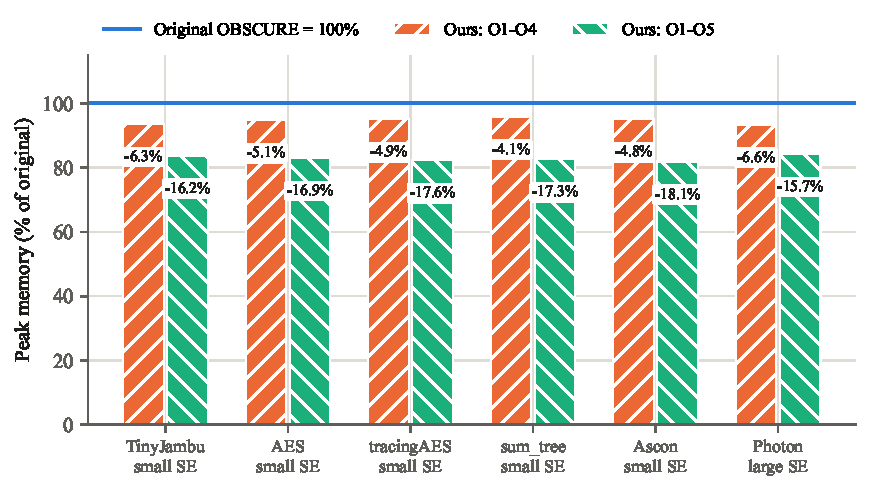
\includegraphics[width=\textwidth]{figures/fig_peak_memory_percent.pdf}
\caption{Peak memory of the optimized compiler relative to the original (100\%).}
\label{fig:peakpct}
\end{figure}

The three repetitions of each small program differed by at most 0.3~MB, so the differences in
Table~\ref{tab:peak} are far above the measurement noise. O1--O4 reduce the peak by
4.1--6.6\%, mainly through O4. Adding O5 reduces it by 15.7--18.1\% in total.

\section{Medium Test Case: PHOTON on the Large SE}
\label{sec:photon}
Photon on the large SE is our medium test case: 47{,}248 high-level instructions, a universalized
circuit of depth 162 and width 14, and about 9.4 minutes per compilation, most of it in the unchanged
clusterizer (Table~\ref{tab:photon}, Figure~\ref{fig:timeline}).

\begin{table}[H]
\centering\small
\caption{Medium test case: Photon, large SE ($l_{in}=l_{out}=32$, $r=160$, $s=128$), seed 1.}
\label{tab:photon}
\begin{tabular}{@{}l r r r@{}}
\toprule
 & Original & O1--O4 & O1--O5\\ \midrule
Peak memory (MB) & 710.5 & 663.5 & \textbf{599.2}\\
Change vs.\ original & --- & $-6.6\%$ & \textbf{\textminus15.7\%}\\
Memory saved (MB) & --- & 47.0 & \textbf{111.3}\\
Wall time (s) & 561.7 & 564.4 & 515.0\\
Final multi-instructions & 20{,}711 & 20{,}711 & 20{,}711\\
Bytecode size (bytes) & 10{,}045{,}209 & 10{,}045{,}209 & 10{,}045{,}209\\
Bytes differing from original & --- & 64 (key header only) & 64 (key header only)\\
Functional tests (large-SE interpreter) & 2/2 & 2/2 & 2/2\\
\bottomrule
\end{tabular}
\end{table}

The bytecodes differ only in the 64 bytes of the sealed key, so the obfuscated program is
\textbf{exactly the same}, and with a large-SE interpreter all three returned the plain C program's
256 output words. Peak memory fell from 710.5~MB to \textbf{599.2~MB} ($-$111.3~MB, 15.7\%).
A second, independent run with the testing utility (Figure~\ref{fig:ss3}) reproduced this result:
710.8~MB $\rightarrow$ 598.2~MB ($-15.8\%$, 112.6~MB saved), identical bytecode and 2/2 functional
tests, so the measurement is repeatable to within about 1~MB.
\screenshot{ss_photon.png}{python3 compare\_mem.py -{}-program Photon -{}-se large -{}-tests 2 -{}-label Photon\_demo}{Testing
utility on the medium test case Photon (large SE), second run: 15.8\% lower peak memory, identical
bytecode, all functional tests passed.\label{fig:ss3}}

In Figure~\ref{fig:timeline} the runs are aligned at the end of clusterization, because the
earlier passes are unchanged and their run-to-run time variation would otherwise shift the
curves. The three curves coincide during universalization (the gates are identical). At the
hand-off to lowering, the O4 curves drop by about 25~MB (released bookkeeping), and during
serialization the O1--O5 curve stays about 110~MB below the original because the universalized
DFG has already been freed.

\begin{figure}[H]
\centering
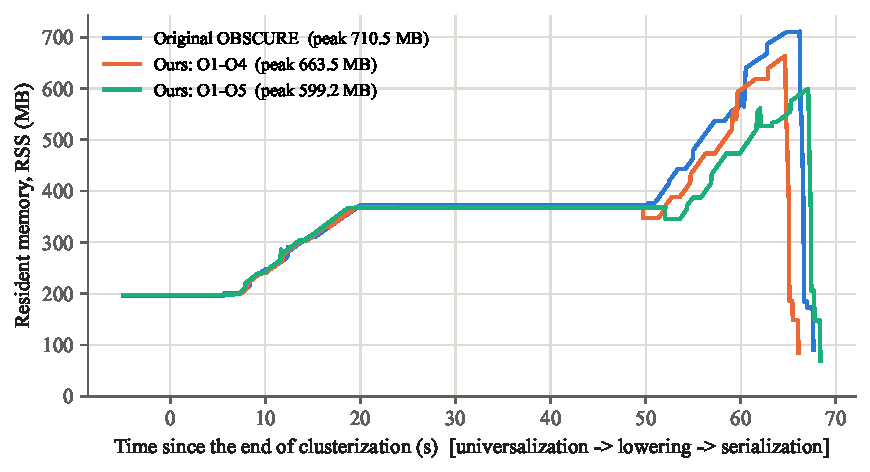
\includegraphics[width=0.8\textwidth]{figures/fig_timeline_Photon_large.pdf}
\caption{Resident memory over time while compiling Photon (large SE).}
\label{fig:timeline}
\end{figure}

\section{Complete Test Suite}
\label{sec:suite}
We ran the testing utility on the test cases of the repository's \code{tests/automated} folder:
49 basic, 4 medium and 6 advanced programs, plus Photon on the large SE (Section~\ref{sec:photon}).
Every case was compiled with the original compiler and with ours using O1--O5
(\code{-opt-all -opt-o5}, seed~1); the bytecodes were compared byte for byte and executed on the
interpreter against the plain C program (two random inputs for basic and medium programs, three for
the advanced ones). Table~\ref{tab:suite} summarizes the outcome.

\begin{table}[H]
\centering\small
\caption{Summary of the complete test suite (O1--O5 against the original compiler, seed 1).}
\label{tab:suite}
\begin{tabular}{@{}l c c c c@{}}
\toprule
Group (folder) & Cases & Same output & Functional tests & Peak-memory change\\ \midrule
Basic (\code{basic}) & 49 & 49/49 & 49/49 & $-0.4\%$ to $-10.2\%$\\
Medium (\code{medium}) & 4 & 4/4 & 4/4 & $-1.6\%$ to $-16.7\%$\\
Advanced (\code{programs}), small SE & 6 & 6/6 & 6/6 & $-16.4\%$ to $-18.6\%$\\
Photon, large SE (medium test case) & 1 & 1/1 & 1/1 & $-15.6\%$ to $-15.8\%$\\ \midrule
\textbf{Total} & \textbf{60} & \textbf{60/60} & \textbf{60/60} & $-0.4\%$ to $-18.6\%$\\
\bottomrule
\end{tabular}
\end{table}

\textbf{All 60 test cases produce exactly the same bytecode as the original compiler and pass every
functional test.}

\subsection{Basic Programs (49)}
The basic programs are very small, so their peak of about 25~MB is mostly the Python interpreter
itself. The largest one, \code{ptr\_alias\_middle\_arith}, saves 5.5~MB ($-10.2\%$).
Table~\ref{tab:basic} lists every case.

\begin{table}[H]
\centering\scriptsize
\caption{All 49 basic test cases (O1--O5, \code{-width 4 -depth 25}, two functional tests each); peak memory in MB. Every case gives the same bytecode as the original.}
\label{tab:basic}
\setlength{\tabcolsep}{3.5pt}
\begin{tabular}{@{}l r r r c@{\hspace{10pt}}l r r r c@{}}
\toprule
Test case & Orig. & Opt. & Change & Func. & Test case & Orig. & Opt. & Change & Func.\\ \midrule
add & 24.8 & 24.7 & $-0.4\%$ & 2/2 & lsl & 25.0 & 24.7 & $-1.2\%$ & 2/2\\
and & 25.0 & 24.6 & $-1.6\%$ & 2/2 & lsr & 25.0 & 24.6 & $-1.6\%$ & 2/2\\
array\_as\_input & 25.0 & 24.6 & $-1.6\%$ & 2/2 & mod & 25.0 & 24.6 & $-1.6\%$ & 2/2\\
array\_as\_input\_nomod & 25.0 & 24.8 & $-0.8\%$ & 2/2 & mul & 25.0 & 24.6 & $-1.6\%$ & 2/2\\
array\_as\_input\_voidfun & 25.0 & 24.7 & $-1.2\%$ & 2/2 & nested\_expr & 25.0 & 24.7 & $-1.2\%$ & 2/2\\
array\_basic & 24.9 & 24.6 & $-1.2\%$ & 2/2 & nested\_expr\_funcall & 25.0 & 24.7 & $-1.2\%$ & 2/2\\
array\_for & 24.9 & 24.5 & $-1.6\%$ & 2/2 & ptr\_alias & 25.1 & 24.8 & $-1.2\%$ & 2/2\\
array\_fun & 25.0 & 24.6 & $-1.6\%$ & 2/2 & ptr\_alias\_middle\_arith & 54.1 & 48.6 & $-10.2\%$ & 2/2\\
array\_funcall & 25.1 & 24.6 & $-2.0\%$ & 2/2 & ptr\_alias\_middle\_array & 25.1 & 24.8 & $-1.2\%$ & 2/2\\
array\_init & 25.1 & 24.6 & $-2.0\%$ & 2/2 & ptr\_alias\_middle\_ptr & 25.0 & 24.7 & $-1.2\%$ & 2/2\\
array\_noinit\_fun & 25.0 & 24.7 & $-1.2\%$ & 2/2 & ptr\_alias\_middle\_ptr\_arr & 25.0 & 24.7 & $-1.2\%$ & 2/2\\
binops & 25.0 & 24.5 & $-2.0\%$ & 2/2 & ptr\_as\_input & 25.1 & 24.7 & $-1.6\%$ & 2/2\\
bitnot & 25.1 & 24.7 & $-1.6\%$ & 2/2 & ptr\_as\_input\_const & 25.0 & 24.6 & $-1.6\%$ & 2/2\\
cmp\_eq & 25.0 & 24.5 & $-2.0\%$ & 2/2 & ptr\_as\_input\_const\_mixed & 25.1 & 24.7 & $-1.6\%$ & 2/2\\
cmp\_lt & 25.0 & 24.6 & $-1.6\%$ & 2/2 & ptr\_basic & 25.0 & 24.7 & $-1.2\%$ & 2/2\\
compound\_asgn & 25.0 & 24.6 & $-1.6\%$ & 2/2 & ptr\_for & 25.0 & 24.6 & $-1.6\%$ & 2/2\\
div & 24.9 & 24.6 & $-1.2\%$ & 2/2 & ptr\_fun & 25.0 & 24.8 & $-0.8\%$ & 2/2\\
for\_complex\_next & 25.0 & 24.5 & $-2.0\%$ & 2/2 & ptr\_late\_assign & 25.0 & 24.6 & $-1.6\%$ & 2/2\\
for\_simple & 25.0 & 24.6 & $-1.6\%$ & 2/2 & ptr\_without\_dereference & 25.0 & 24.7 & $-1.2\%$ & 2/2\\
for\_with\_var & 25.0 & 24.6 & $-1.6\%$ & 2/2 & static\_var\_becomes\_dynami & 24.9 & 24.7 & $-0.8\%$ & 2/2\\
funs & 25.0 & 24.6 & $-1.6\%$ & 2/2 & sub & 25.0 & 24.7 & $-1.2\%$ & 2/2\\
funs\_complex & 25.0 & 24.8 & $-0.8\%$ & 2/2 & ternary\_if & 24.9 & 24.8 & $-0.4\%$ & 2/2\\
funs\_nested\_calls & 25.1 & 24.7 & $-1.6\%$ & 2/2 & ternary\_if\_nested & 25.0 & 24.7 & $-1.2\%$ & 2/2\\
funs\_twice\_called & 25.0 & 24.7 & $-1.2\%$ & 2/2 & xor & 25.0 & 24.7 & $-1.2\%$ & 2/2\\
int\_hexa & 25.0 & 24.7 & $-1.2\%$ & 2/2 & & & & &\\
\bottomrule
\end{tabular}
\end{table}

\subsection{Medium Programs (4)}
Figure~\ref{fig:ssmed} shows the four medium programs. \code{msb32\_from\_binmul} saves 20.3~MB
($-16.7\%$); the other three save 1.6--3.7\%.
\screenshot{ss_suite_medium.jpeg}{}{Testing utility on the four medium test cases (O1--O5): same
output and 2/2 functional tests for every case.\label{fig:ssmed}}

\subsection{Advanced Programs (6) and Photon}
Figure~\ref{fig:ssadv} shows the six advanced programs (small SE). They save 16.4--18.6\%, in line
with Table~\ref{tab:peak}; \code{findmax\_tree} gives the largest saving ($-18.6\%$).
Figure~\ref{fig:ssph2} shows Photon on the large SE: 710.7 $\rightarrow$ 599.7~MB ($-15.6\%$,
111.0~MB saved), identical bytecode and 3/3 functional tests.
\screenshot{ss_suite_advanced.jpeg}{}{Testing utility on the six advanced test cases (small SE,
O1--O5): same output and 3/3 functional tests for every case.\label{fig:ssadv}}
\screenshot{ss_photon_run2.jpeg}{}{Testing utility on Photon (large SE): 15.6\% lower peak memory, identical bytecode, 3/3 functional tests.\label{fig:ssph2}}

\section{Where the Memory Is Saved}
\label{sec:phase}
The per-phase memory recorded by the utility explains the result (Figure~\ref{fig:timeline}). Up to the end of
universalization all three versions use the same memory: the gates are the output and are
identical. The savings appear afterwards. O4 lowers the memory during lowering, because the
released bookkeeping no longer sits under the scheduler's data. O5 lowers the memory during
serialization, the phase where the original reaches its peak, because the universalized DFG is
freed before the serializer allocates the bytecode. 

\section{Compile Time}
The optimizations do not slow down compilation: with O1--O5 the whole compilation took 5.9 vs.\
5.6~s (TinyJambu), 12.1 vs.\ 11.7~s (AES), 71.7 vs.\ 71.7~s (Ascon) and 515 vs.\ 562~s (Photon; the
difference is in the unchanged clusterizer). On the wide sum\_tree (width 186), O3 halves the
permutation-network step (11.4 $\rightarrow$ 5.8~s) by removing the per-gate copies of the wire list.

\section{Stretch Goal: Width-Balancing Layering}
With \code{-opt-layering} the guard estimated a width of 21 for the original ASAP layering and 6
for the balanced one on Ascon (small SE), and adopted the balanced layering. Table~\ref{tab:layer}
compares it with the original and with O1--O5.

\begin{table}[H]
\centering\small
\caption{Stretch goal on Ascon (small SE). The layering run produces a different program.}
\label{tab:layer}
\begin{tabular}{@{}l r r r@{}}
\toprule
 & Original & O1--O5 & O1--O5 + layering\\ \midrule
Peak memory (MB) & 962.5 & 788.3 & \textbf{157.3}\\
Change vs.\ original & --- & $-18.1\%$ & \textbf{\textminus83.7\%}\\
Circuit depth $\times$ width & $317 \times 21$ & $317 \times 21$ & $317 \times 6$\\
Final multi-instructions & 120{,}188 & 120{,}188 & 20{,}033\\
Bytecode size (bytes) & 17{,}264{,}565 & 17{,}264{,}565 & 2{,}939{,}508\\
Wall time (s) & 71.7 & 71.7 & 28.0\\
Same bytecode as original & --- & yes & no (by design)\\
Functional tests & 3/3 & 3/3 & 3/3\\
\bottomrule
\end{tabular}
\end{table}

Reducing the width from 21 to 6 shrinks every permutation network, so the number of
multi-instructions falls by a factor of six and the peak memory by 83.7\%. The obfuscated program
is different and is therefore not covered by the identical-output guarantee; it is still
rectangular with the same depth, and it produced correct results in all functional tests. In our
group's earlier study the guard adopted the balanced layering in 9 of 36 configurations and kept
the original program in the others.

\section{Comparative Analysis: Original versus Optimized}
\begin{table}[H]
\centering\small
\caption{Qualitative and quantitative comparison.}
\label{tab:compare}
\footnotesize
\begin{tabularx}{\textwidth}{@{}l X X@{}}
\toprule
Aspect & Original OBSCURE & Optimized (O1--O5)\\ \midrule
Obfuscated output / security & reference; Theorem 1 of \cite{obscure} & byte-identical, so unchanged\\
Peak memory & reference & 15.7--18.1\% lower on all tested programs\\
Routing networks & all columns at once, copied twice & generated lazily, compact arrays\\
Gate application & whole wire list copied per gate & only the gate's window updated\\
Bookkeeping, HLIR, DFG & kept until the end of compilation & released after last use (O4, O5)\\
Reproducibility, measurement & non-deterministic; \code{-stats} only & \code{-seed}; \code{-profile-mem}, \code{compare\_mem.py}\\
\bottomrule
\end{tabularx}
\end{table}

\textbf{Comparison with our group's earlier study.} On 9 programs and all 4 SE sizes (36
configurations, another machine and Python 3.13), O1--O4 gave byte-identical output everywhere and
0.2--9.6\% (median 5.9\%) lower peak memory, consistent with the 4.1--6.6\% measured here; O5 adds a
further and larger saving.

\section{Discussion and Threats to Validity}
\textbf{Bounded gain:} after universalization the gate objects are the output, so they cannot be
removed without changing the bytecode; O1--O5 remove only what is \emph{not} output.
\textbf{Machines:} repeated measurements agree to within 1.5~MB, and the relative reductions agree
with our earlier study on another machine.
\textbf{Coverage:} 60 test cases were tested; the heaviest configurations (3--5~GB) were not rerun
in this phase.
\textbf{Deterministic mode:} it is applied to both compilers and fixes only the iteration order.

% ---------------------------------------------------------------- Chapter 5
\chapter{Conclusion and Future Work}

\section{Conclusion}
This project studied the universalization pass of the OBSCURE obfuscator and reduced the memory
used by the compiler without changing the obfuscated output. Profiling showed that most of the
memory of universalization is the routing gates, i.e.\ the output itself, and that the peak of
the whole compilation is reached during serialization. Accordingly, we implemented five
optimizations that remove only memory that is not part of the output: sparse bookkeeping (O1),
lazy routing generation (O2), in-place gate application (O3), a compact hand-off to lowering (O4)
and early release of finished program representations (O5).

A new testing utility compares the original and the optimized compiler on the same input. On
all 60 test cases (49 basic, 4 medium, 6 advanced programs and Photon on the large SE), the
optimized compiler produced byte-identical bytecode and passed every functional test.
With O1--O5 the peak memory of the whole compiler decreased by 15.7--18.1\%, including the medium
test case Photon on the large SE (710.5~MB $\rightarrow$ 599.2~MB), and O3 halved the
permutation-network time on wide programs. The optional width-balancing layering showed that much
larger savings are possible when the circuit itself may change.

\section{Future Work}
\begin{itemize}
\item \textbf{Compact IR objects.} The gate objects (MLMI, MLS, HLI, MemOperand) are ordinary
      Python objects with per-instance dictionaries. Declaring \code{\_\_slots\_\_} \cite{pyslots}
      or storing operands as integer identifiers would shrink the remaining memory while keeping
      the output identical.
\item \textbf{Streaming.} Lowering and serializing finished layers while later layers are still
      being built would make the peak depend on the width rather than on the depth; this requires
      changing the scheduler, which currently works on the whole graph.
\item \textbf{Better layering.} Exact width-minimizing layering for small programs (integer
      programming) or Coffman--Graham layering \cite{coffman}, and a guard that also accepts
      smaller gains.
\item \textbf{Time on large SEs.} O2's conversion of every column to an array costs time with very
      wide gates; making it optional per SE size would remove this overhead.
\item \textbf{Wider evaluation.} Repeat the full 36-configuration study with O5 on more machines.
\end{itemize}

% ---------------------------------------------------------------- References
\clearpage
\phantomsection
\addcontentsline{toc}{chapter}{References}
\renewcommand{\bibname}{References}
\begingroup\small\setstretch{1.1}
\begin{thebibliography}{99}
\setlength{\itemsep}{1pt}
\bibitem{obscure} D.~Mercadier, V.~S.~Nguyen, M.~Rivain and A.~Udovenko, ``OBSCURE: Versatile
  software obfuscation from a lightweight secure element,'' \emph{IACR Transactions on
  Cryptographic Hardware and Embedded Systems}, vol.~2024, no.~2, pp.~588--629, 2024,
  doi:10.46586/tches.v2024.i2.588-629.
\bibitem{obscuregit} CryptoExperts, ``OBSCURE source code,''
  \url{https://github.com/CryptoExperts/OBSCURE}.
\bibitem{chow} S.~Chow, P.~Eisen, H.~Johnson and P.~C.~van~Oorschot, ``White-box cryptography and
  an AES implementation,'' in \emph{Selected Areas in Cryptography (SAC 2002)}, LNCS~2595,
  Springer, 2003, pp.~250--270.
\bibitem{billet} O.~Billet, H.~Gilbert and C.~Ech-Chatbi, ``Cryptanalysis of a white box AES
  implementation,'' in \emph{Selected Areas in Cryptography (SAC 2004)}, LNCS~3357, Springer,
  2005, pp.~227--240.
\bibitem{bgi} B.~Barak, O.~Goldreich, R.~Impagliazzo, S.~Rudich, A.~Sahai, S.~Vadhan and
  K.~Yang, ``On the (im)possibility of obfuscating programs,'' in \emph{Advances in Cryptology --
  CRYPTO 2001}, LNCS~2139, Springer, 2001, pp.~1--18.
\bibitem{jls} A.~Jain, H.~Lin and A.~Sahai, ``Indistinguishability obfuscation from well-founded
  assumptions,'' in \emph{Proc.\ 53rd ACM Symposium on Theory of Computing (STOC)}, 2021,
  pp.~60--73.
\bibitem{gis} V.~Goyal, Y.~Ishai, A.~Sahai, R.~Venkatesan and A.~Wadia, ``Founding cryptography
  on tamper-proof hardware tokens,'' in \emph{Theory of Cryptography Conference (TCC 2010)},
  LNCS~5978, Springer, 2010, pp.~308--326.
\bibitem{sgx} V.~Costan and S.~Devadas, ``Intel SGX explained,'' IACR Cryptology ePrint Archive,
  Report 2016/086, 2016.
\bibitem{valiant} L.~G.~Valiant, ``Universal circuits (preliminary report),'' in \emph{Proc.\
  8th ACM Symposium on Theory of Computing (STOC)}, 1976, pp.~196--203.
\bibitem{ks16} \'A.~Kiss and T.~Schneider, ``Valiant's universal circuit is practical,'' in
  \emph{Advances in Cryptology -- EUROCRYPT 2016}, LNCS~9665, Springer, 2016, pp.~699--728.
\bibitem{benes} V.~E.~Bene\v{s}, ``Optimal rearrangeable multistage connecting networks,''
  \emph{Bell System Technical Journal}, vol.~43, no.~4, pp.~1641--1656, 1964.
\bibitem{waksman} A.~Waksman, ``A permutation network,'' \emph{Journal of the ACM}, vol.~15,
  no.~1, pp.~159--163, 1968.
\bibitem{bernstein} D.~J.~Bernstein, ``Verified fast formulas for control bits for permutation
  networks,'' IACR Cryptology ePrint Archive, Report 2020/1493, 2020.
\bibitem{sugiyama} K.~Sugiyama, S.~Tagawa and M.~Toda, ``Methods for visual understanding of
  hierarchical system structures,'' \emph{IEEE Transactions on Systems, Man, and Cybernetics},
  vol.~11, no.~2, pp.~109--125, 1981.
\bibitem{healy} P.~Healy and N.~S.~Nikolov, ``How to layer a directed acyclic graph,'' in
  \emph{Graph Drawing (GD 2001)}, LNCS~2265, Springer, 2002, pp.~16--30.
\bibitem{graham} R.~L.~Graham, ``Bounds on multiprocessing timing anomalies,'' \emph{SIAM
  Journal on Applied Mathematics}, vol.~17, no.~2, pp.~416--429, 1969.
\bibitem{coffman} E.~G.~Coffman and R.~L.~Graham, ``Optimal scheduling for two-processor
  systems,'' \emph{Acta Informatica}, vol.~1, pp.~200--213, 1972.
\bibitem{kahn} A.~B.~Kahn, ``Topological sorting of large networks,'' \emph{Communications of the
  ACM}, vol.~5, no.~11, pp.~558--562, 1962.
\bibitem{pygc} Python Software Foundation, ``gc --- Garbage Collector interface,'' \emph{Python
  3.12 Documentation}, \url{https://docs.python.org/3.12/library/gc.html}.
\bibitem{tracemalloc} Python Software Foundation, ``tracemalloc --- Trace memory allocations,''
  \emph{Python 3.12 Documentation}, \url{https://docs.python.org/3.12/library/tracemalloc.html}.
\bibitem{pyslots} Python Software Foundation, ``Data model: \_\_slots\_\_,'' \emph{The Python
  Language Reference}, \url{https://docs.python.org/3.12/reference/datamodel.html}.
\bibitem{getrusage} ``getrusage(2) --- get resource usage,'' \emph{Linux Programmer's Manual},
  \url{https://man7.org/linux/man-pages/man2/getrusage.2.html}.
\bibitem{procfs} ``proc\_pid\_status(5),'' \emph{Linux Programmer's Manual},
  \url{https://man7.org/linux/man-pages/man5/proc_pid_status.5.html}.
\bibitem{libsodium} F.~Denis et al., ``Sealed boxes,'' \emph{libsodium documentation},
  \url{https://doc.libsodium.org/public-key_cryptography/sealed_boxes}.
\bibitem{pycparser} E.~Bendersky, ``pycparser: Complete C99 parser in pure Python,''
  \url{https://github.com/eliben/pycparser}.
\bibitem{aes} National Institute of Standards and Technology, ``Advanced Encryption Standard
  (AES),'' FIPS PUB 197, 2001.
\bibitem{ascon} C.~Dobraunig, M.~Eichlseder, F.~Mendel and M.~Schl\"affer, ``Ascon v1.2:
  Lightweight authenticated encryption and hashing,'' \emph{Journal of Cryptology}, vol.~34,
  no.~3, 2021.
\bibitem{tinyjambu} H.~Wu and T.~Huang, ``TinyJAMBU: A family of lightweight authenticated
  encryption algorithms,'' submission to the NIST Lightweight Cryptography project, 2019.
\bibitem{photon} J.~Guo, T.~Peyrin and A.~Poschmann, ``The PHOTON family of lightweight hash
  functions,'' in \emph{Advances in Cryptology -- CRYPTO 2011}, LNCS~6841, Springer, 2011,
  pp.~222--239.
\end{thebibliography}
\endgroup

% ---------------------------------------------------------------- Appendices
\end{document}
